\documentclass[14pt,a4paper]{report}
\usepackage[utf8]{inputenc}
%Idioma
\usepackage[spanish]{babel}
\spanishdecimal{.}
%Para expresiones matematicas
\usepackage{titlesec}
\usepackage{amsmath}
\usepackage{amsfonts}
\usepackage{amssymb}
\usepackage{amstext}
\usepackage{mathtools}
\usepackage{mathrsfs}
\usepackage{physics}
%Imagenes
\usepackage{graphicx}
\usepackage{color}
%Para dibujar
\usepackage{tikz}
\usetikzlibrary{arrows.meta}
\usetikzlibrary{decorations.markings}
\usetikzlibrary{babel,patterns,snakes}
\usetikzlibrary{shapes.callouts}
\usetikzlibrary{calc,patterns,angles,quotes}
\usetikzlibrary{shadings}
%Cajas con colores
\usepackage{tcolorbox}
\tcbuselibrary{theorems}
%Ejemplo de lo anterior
%\begin{equation}
% a x^2 + bx + c = 0 \rightarrow
%\tcboxmath[colback=magenta!25!white,colframe=magenta, title=Solución]
%{x = \frac{-b\pm\sqrt{b^2-4ac}}{2a}}  
%\end{equation}
%
%Estilo fancy
\usepackage{fancyhdr}
%Interlineado y margenes y poco mas
\usepackage{setspace}
\usepackage{parskip}
\usepackage{multicol}
\usepackage[left=2.5cm,right=2.5cm,top=2.5cm,bottom=2.5cm]{geometry}
%Empieza documento
\begin{document}
%Cajas comentadas 
\newcommand{\commentedbox}[2]{%
  \mbox{
    \begin{tabular}[t]{@{}c@{}}
    $\boxed{\displaystyle#1}$\\
    #2
    \end{tabular}%
  }%
}
%Definimos el estilo de las paginas
\pagestyle{fancy}
\lhead{\itshape Cursos  - MCD}
\rhead{Proyecto Individual - Parte 1}
\Large{Matemáticas - \textit{Redes Neuronales}}\\
\normalsize
Rodolfo Armando Jaramillo Ruiz\\
31 de Mayo de 2023\\
\section*{¿Qué son las redes neuronales?}
\textit{A neural network is a massively parallel distributed processor made up of simple processing units, which has a natural propensity for storing experiential knowledge and making it available for use. It resembles the brain in two respects:}

\begin{enumerate}
\item \textit{Knowledge is acquired by the network from its environment through a learning process.}
\item \textit{Interneuron connection strengths, known as synaptic weights, are used to store the acquired knowledge.}
\end{enumerate}

— Haykin, S. (1999). Neural Network a Comprehensive Foundation (p. 2).

Esta es la definición de lo que es una red neuronal desde la perspectiva computacional. En síntesis, una red neuronal es un conjunto de operadores sencillos que trabajan en conjunto para almacenar conocimiento obtenido de su interacción con el entorno.

La idea del cómputo a través de modelos como el descrito anteriormente es tener un sistema capaz de aprender a través de \textit{inputs} ambientales, adaptarse y resolver problemas de manera más flexible.

\subsection*{Neurona Artificial}

El modelo de una neurona artificial es el siguiente:

\begin{figure}[h]
  \centering
  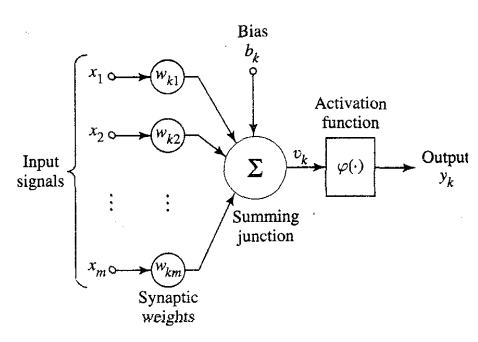
\includegraphics[scale=0.8]{../artificial-neural.png}
  \caption{Haykin, S. (1999). Neural Network a Comprehensive Foundation (p. 11)}
  \label{fig:neural-network}
\end{figure}

Leído de izquierda a derecha, se puede ver que los \textit{inputs signals} entran desde los nodos de origen. El valor que entra por estos nodos es multiplicados por un factor que se llama \textit{Synaptic weights} o pesos sinápticos. Estos productos entran a un nodo referido como \textit{Summing junction}. Además se agrega el \textit{bias} o sesgo. La suma, entonces, es la siguiente:
$$
v_k = \sum_{j=1}^{m} w_{kj}x_{j}+b_{k}
$$
Esta expresión nos dice que si tenemos $m$ nodos origen por donde los datos entran, estos nueve son multiplicados por sus pesos respectivos, se suman todos estos, lo que es una suma ponderada, y se agrega el \textit{bias} como $b_{k}$ para obtener el valor $v_{k}$ de una neurona $k$.

También se puede ver al \textit{bias} como un \textit{input} que siempre $x_{0} = 1$ donde el \textit{bias} sea un peso más, de forma que que $w_{k0}=b_k$, obteniendo entonces una expresión diferentes para $v_k$:
$$
v_k = \sum_{j=0}^{m} w_{kj}x_{j}
$$

Que le corresponde el siguiente diagrama:

 \begin{figure}[h]
  \centering
  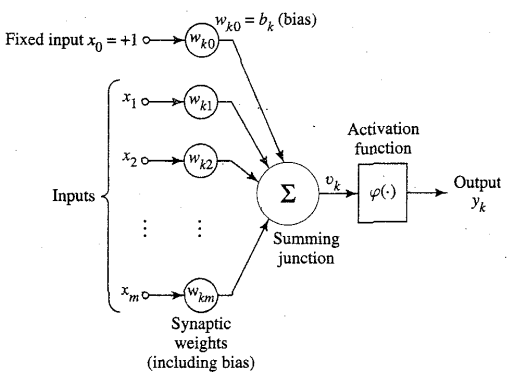
\includegraphics[scale=0.8]{../artificial-neural-fixed-input.png} 
  \caption{Haykin, S. (1999). Neural Network a Comprehensive Foundation (p. 35)}
  \label{fig:neural-network}
\end{figure}


Luego, tenemos que pasar este valor $v_{k}$ por la función de activación. Al pasar la señal que sale del \textit{summing junction} por la función de activación determina si la neurona debe mandar la señal o no, y en que medida. Existe varias funciones de activación que se usan en diferentes partes de la redes y en diferentes tipos de redes. Dependiendo de la función que se use, el desempeño de la red en sus tareas será diferente, se tiene que elegir bien el tipo de función que se usa y en donde, para poder tener buenos resultados. Un ejemplo de función de activación es la función sigmoide, que limita el \textit{output} en el intervalo $[0,1]$
$$
\varphi(v_{k})=\frac{1}{1+e^{-av_{k}}}
$$
 \begin{figure}[h]
  \centering
  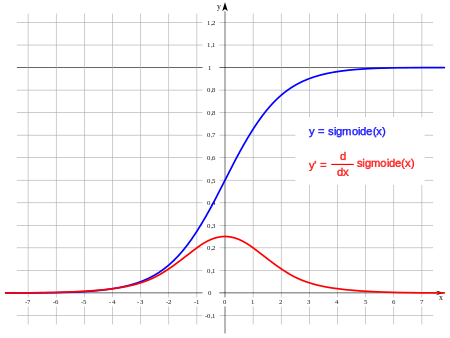
\includegraphics[scale=0.4]{../sigmoide.png}
  \caption{Gráfica de una función sigmoide y su derivada}
  \label{fig:neural-network}
\end{figure}

El \textit{output} de la neurona sería entonces $$y_{k}=\phi(v_{k})$$

\subsection*{Ejemplos de usos y arquitecturas}
Se enumeran ejemplos del uso de Redes Neuronales en nuestra interacción con la tecnología:
\begin{enumerate}


\item En redes sociales se usa para analizar el comportamiento del usuario y mostrar contenido que lo retenga dentro de la aplicación lo más posible. A consideración personal, \textit{TikTok} es uno de los grandes exponentes de un, coloquialmente llamado, "algoritmo de recomendación" poderoso.
\item La existencia de cámaras de seguridad que sean capaz de identificar a personas buscadas es gracias al reconocimiento de imágenes hecho a través de redes neuronales.
\item Dentro de los vídeojuegos se trabaja con agentes inteligentes entrenados usando redes neuronales.
\end{enumerate}

En general se pueden, se puede pensar en tres arquitecturas de redes neuronales para que son fundamentalmente diferentes (Haykin, 1999):\\
\begin{enumerate}


\item Redes Neuronales de una sola capa o \textit{Single-Layer}: Consta solamente de una capa de \textit{inputs} y una capa de \textit{outputs}, sin tener capas ocultas. Se limitan a resolver principalmente para problemas de clasificación binaria.

 \begin{figure}[h]
  \centering
  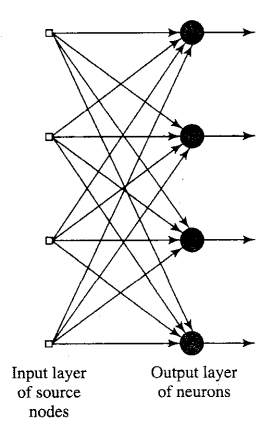
\includegraphics[scale=0.6]{../single-layer-NN.png} 
  \caption{Haykin, S. (1999). Neural Network a Comprehensive Foundation (p. 21)}
  \label{fig:neural-network}
\end{figure}
 

\item Redes Neuronales multicapa o \textit{Multilayer}: Se puede pensar que teniendo una red \textit{Single-Layer} se pueden romper las conexiones entre los nodos de origen y las neuronas para conectar en medio de ellas una capa de neuronas ocultas, volviendo multicapa a la red. Se pueden agregar más de una capa oculta a la red. Sirve para extraer información más profunda de los datos. Se usan para los problemas que involucran reconocimiento de patrones, procesamiento de imágenes. El costo computacional de esta arquitectura es más alto y requiere una gran cantidad de datos para evitar un sobreajuste.

 \begin{figure}[h]
  \centering
  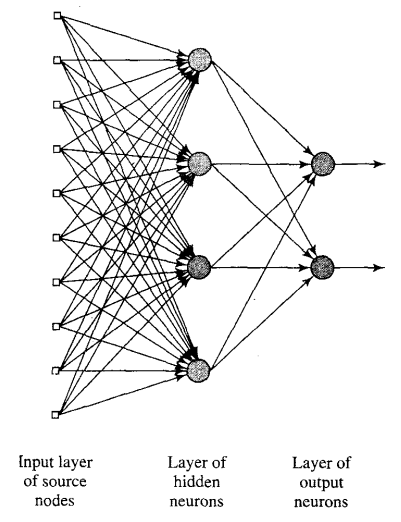
\includegraphics[scale=0.6]{../multilayer-NN.png} 
  \caption{Haykin, S. (1999). Neural Network a Comprehensive Foundation (p. 22)}
  \label{fig:neural-network}
\end{figure}


\item Redes Neuronales Recurrentes o \textit{Recurrent Networks}: Esta estructura de redes se puede ver como una sola capa que se retroalimenta a sí misma, usando los \textit{outputs} de sus nodos como \textit{inputs}. Lo especial de esta arquitectura es especial porque permite a la red aprender a capturar dependencias temporales o contextuales. La clave es su capacidad para mantener una "memoria" interna, también llamada estado oculto, que se actualiza a medida que procesa cada elemento de la secuencia. Esta memoria interna le permite aprender a capturar estas características.
 
  \begin{figure}[h]
  \centering
  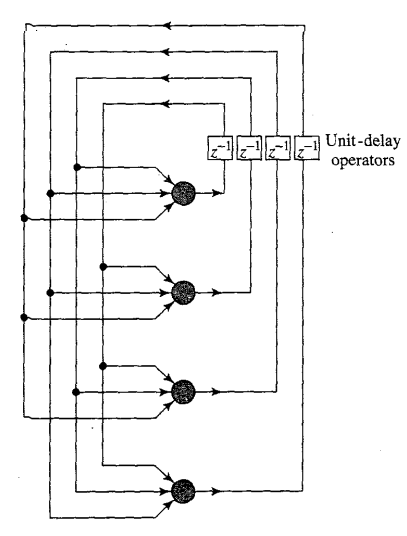
\includegraphics[scale=0.6]{../recurrent-NN.png} 
  \caption{Haykin, S. (1999). Neural Network a Comprehensive Foundation (p. 23)}
  \label{fig:neural-network}
\end{figure}


Estas arquitecturas se pueden combinar para crear estructuras con mucho potencial de aprendizaje, estas tres son solo la generalidad.
\end{enumerate}

\section*{Backpropagation - ¿Cómo aprenden una red neuronal?}

El siguiente diagrama explica de manera simple el como se entrena una red neuronal usando \textit{Backpropagation}. Este nombre es una contracción de \textit{backward propagation} y es importante apuntar que este nombre es el del algoritmo mostrado en el diagrama, usado para entrenar redes neuronales, y que también hace referencia al paso cuatro en el diagrama. Todo quedará más claro en la explicación del algoritmo que sigue a continuación.

 \begin{figure}[h]
  \centering
  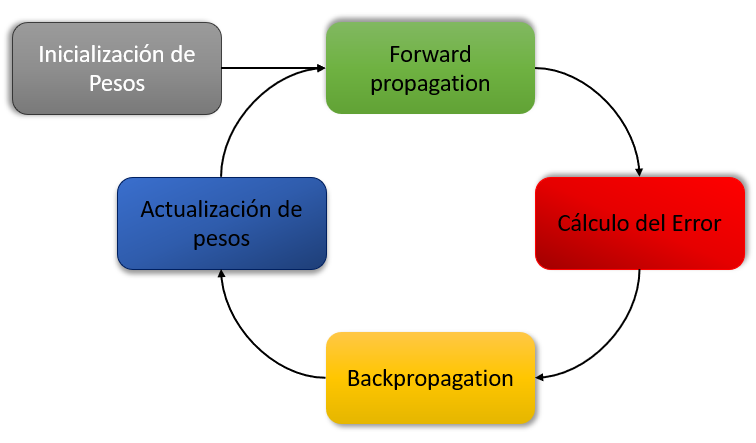
\includegraphics[scale=0.7]{../diagrama-NN.png} 
  \caption{Diagrama de entrenamiento de una red neuronal}
  \label{fig:neural-network}
\end{figure}


Se describen los pasos en cada punto del diagrama.
\begin{enumerate}


\item Inicialización de pesos: Se tiene que a cada entrada le corresponde un peso distinto, todos estos pesos se pueden acomodar en un vector de la forma:$$\textbf{w}=[w_0, w_1, w_2, ..., w_m]$$ para cada neurona con $m$ entradas. Se dan valores iniciales para este vector. Se recomienda usar $0$ o valores cercanos a este. Por ejemplo:$$\textbf{w}=[0.1, 0.05, ..., 0.15]$$

\item \textit{Fordward Propagation}: Se reciben los inputs y se hace la suma ponderada junto con el \textit{bias} para obtener $v_k$ y obtener el output con la función de activación. Retomando el funcionamiento de la neurona artificial, dentro del \textit{Summing junction} ocurre el producto punto entre el vector de pesos y el vector de \textit{inputs}, siendo este último de la siguiente forma
$$
\textbf{x}=[1, x_1, x_2, ..., x_m]
$$
Recordando que el elemento en la posición 0 es el \textit{fixed input} que corresponde al \textit{bias}. El producto punto entra en la función de activación (retomaré la función sigmoide para efectos de la explicación) por lo que el \textit{output} de cada neurona sería como el siguiente.
$$
y_k = \varphi(\textbf{x}\cdot\textbf{w})=\frac{1}{1+e^{-a(\textbf{x}\cdot\textbf{w})}}
$$

\item Cálculo del error: una vez obtenido el output se calcula el error del resultado obtenido por la red y el resultado exacto de los datos de entrenamiento. Hay varias formas de calcular este error, para la explicación usaré en el error cuadrático medio (MSE). Este error es el siguiente 
$$\varepsilon = \frac{1}{n} \sum_{n}(y_{\textbf{w}}-y_{real})^{2}$$ 
Siendo $n$ la cantidad de datos de ejemplo, y $y_{\textbf{w}}$ el \textit{output} obtenido por esta combinación de pesos \textbf{w}. Este calculo nos permite tomar más en cuenta las diferencias o errores que sean más grande que uno mientras minimiza los error pequeños.

\item \textit{Backpropagation}: En esta fase se la contribución de cada peso al error total del \textit{output}, haciendo la derivada de $\varepsilon$ con respecto a cada peso. Es decir, el gradiente del error con respecto a los pesos: 
$$\nabla_{\text{w}}\varepsilon = [\frac{\partial\varepsilon}{\partial w_{1}},\frac{\partial\varepsilon}{\partial w_{2}},...,\frac{\partial\varepsilon}{\partial w_{m}}]$$ 
Donde las derivadas son las siguientes para el MSE:
$$\frac{\partial\varepsilon}{\partial w_{i}}=\frac{2}{n} \sum_{n}(y_{\textbf{w}}-y_{real})\cdot \dfrac{\partial y_{\textbf{w}}}{\partial w_{i}}$$.

Se uso la regla de la cadena de esta forma:
$$
\frac{\partial\varepsilon}{\partial w_{i}}=\dfrac{\partial \varepsilon}{\partial y_{\textbf{w}}}\dfrac{\partial y_{\textbf{w}}}{\partial w_{i}}
$$ 

La expansión de derivadas se puede extender mucho más, ya que el \textit{output} de la red es al final una serie de funciones anidadas, por lo que esta última derivada tiene dentro de sí una cadena de derivadas que depende de como sea la función de activación de las neuronas artificiales y como estén conectadas entre sí en la arquitectura interna de la red.

\item Actualización de pesos: Al final todo se trata de optimizar, lo que se quiere es que el error sea el mínimo, por lo que el gradiente del error tiene que disminuir, los pesos tienen que  apuntando a disminuir cada vez más el error. Siendo este el propósito se tiene que se puede recurrir a varios métodos donde se actualicen los pesos de manera que el error sea cada vez menor. El método que voy a presentar será el descenso de gradiente, la forma de hacer este cambio es la siguiente $$\textbf{w}\leftarrow\textbf{w}-\eta\nabla_{\text{w}}\varepsilon$$ Se puede ver que lo que hace esta actualización es tomar los valores del vector $\textbf{w}$ y cambiarlos en dirección donde donde el gradiente disminuye, esto apoyado por un factor que reescala este cambio en los pasos para que evitar situaciones como entrar a un ciclo donde en nunca se llega a un mínimo global o se queda atrapado en un mínimo local.

\end{enumerate}

Una vez actualizados los pesos se vuelve al paso 2 de manera cíclica hasta que el error sea lo suficiente pequeño.

\section*{Problema: Obtener paletas de colores de una imagen.}

El problema consiste en tomar una imagen como input y que el output sea una paleta de colores de la imagen. Mi interés radica en trabajar con una red neuronal convolucional y pienso que sería un ejercicio sencillo para comenzar a trabajar en el procesamiento de imágenes y trabajar más a futuro con el procesamiento de imágenes con otros propósitos.

Se muestra un ejemplo de lo que se busca:

 \begin{figure}[h]
  \centering
  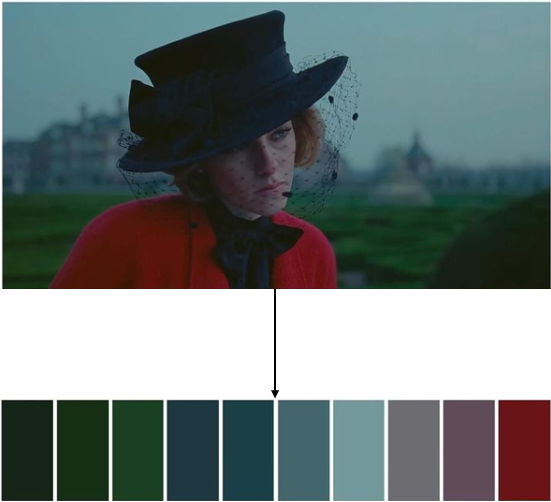
\includegraphics[scale=0.5]{../cinema-pallete.png} 
  \caption{Frame de Spencer (2021) - \textit{@CinemaPalettes} en \textit{Facebook}}
  \label{fig:neural-network}
\end{figure}

Una herramienta que use un modelo entrado para obtener una paleta de colores de una imagen puede ser de gran utilidad para fotógrafos, diseñadores y otros artistas. Los "otros propósitos" hacen referencia a los usos en áreas del diagnostico medico, control de calidad industrial, y más variedad de problemas que se pueden solucionar usando herramientas de procesamiento de  eficientes.

Las redes neuronales convolucionales son una variación de una arquitectura denominada perceptron multicapa, con un cambio inspirado en como funciona la corteza visual del cerebro. La aplicación de esta red es sobre matrices bidimensionales, por lo que si tratamos una imagen como lo que es; una matriz de pixeles, donde cada pixel se le puede asignar una un valor de RGB, entonces se tienen los \textit{inputs} de la red. Un desarrollo más completo de como es el funcionamiento de las redes neuronales convolucionales se hará más adelante en el proyecto.

\end{document}